%!TEX encoding = UTF-8 Unicode
% !TeX spellcheck = en_GB
%%%%%%%%%%%%%%%%%%%%%%%%%%%%%%%%%%%%%%
\chapter{ Overview of Higgs production at colliders }\label{chap:overviewSingleHiggs}
%%%%%%%%%%%%%%%%%%%%%%%%%%%%%%%%%%%%%%
The production of the Higgs boson at the LHC occurs via four distinct processes: gluon fusion~(ggF), vector boson fusion~(VBF), associated production with electroweak boson~($Vh$) and the production with top ( and anti-top) pair~($th / t \bar th$). It should be noted that sometimes the ggF category will include the quark anti-quark annihilation, but this is negligible in the SM, but becomes important for significant modifications of light Yukawa couplings. These process are illustrated in~\autoref{fig:singlehiggs}, and their details were summarised in~\autoref{table:singlehiggs}. All of these four channels have been observed at the LHC with $>5 \sigma$ precision. \\ 
Since the experimental measurements of this Higgs were discussed previously in~\autoref{sec:Higgscoupl}, the aim of this chapter is to provide an overview of the current theoretical status of these channels in~\autoref{sec:singlehiggschannels}. I will then conclude this overview in~\autoref{sec:singlehiggsconc}. 
\begin{table}[htbp!]
	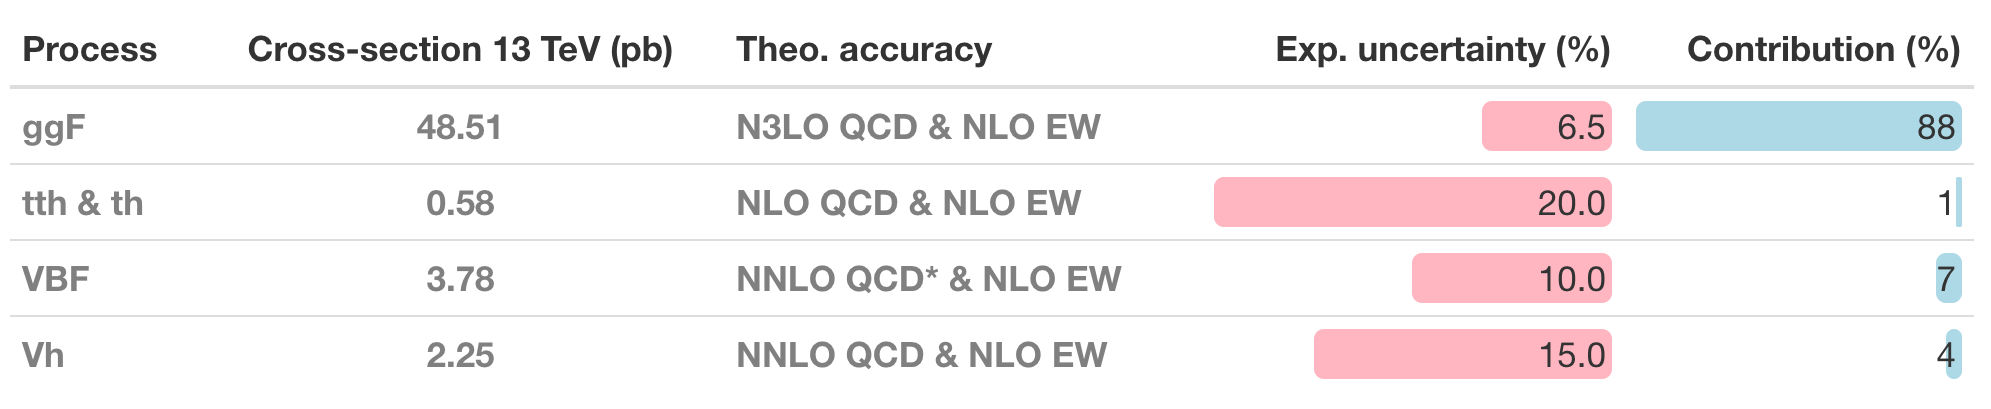
\includegraphics[width=1\textwidth]{single_higgs_table}
	\caption{ Summery  of the Higgs \label{table:singlehiggs} }
\end{table}
\begin{figure}[htbp!]
	\begin{center}
		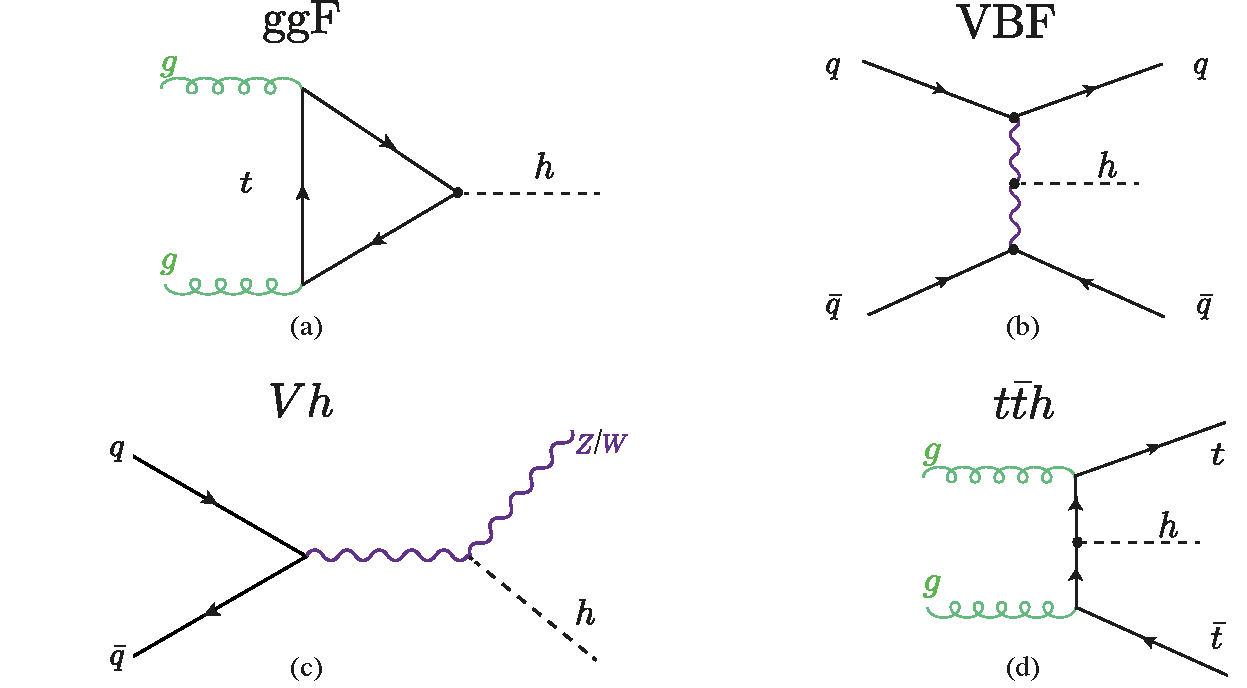
\includegraphics[width=.75\textwidth]{figures/single_higgs}
		\caption{$\sim88$\% ggF, $\sim 7$\% VBF,$\sim 4$\% $Vh$,$\sim1$ $t\bar t h$.  \label{fig:singlehiggs} }
	\end{center}
\end{figure}
\section{Current status of the Higgs production channels  \label{sec:singlehiggschannels}  }
\subsection{Gluon fusion}
The ggF channel has the highest cross-section amongst the Higgs production channels, and consequently has the lowest experimental uncertainties. In order to increase the precision of the channel, Higher order corrections need to be included. The current state-of-the-art theoretical computation for the Higgs inclusive cross-section is N$\,^3$LO in QCD and NLO in EW~\cite{Bonetti:2018ukf}. A full differential cross-section for the final state $ gg \to h \to \gamma \gamma$ has been computed recently to~N$\,^3$LO in QCD for the kinematic variables~$y_h, \ y_{\gamma_1},\ y_{\gamma_2},\ \Delta y_{1,2}$ using the projection-to-born method~\cite{Chen:2021isd}. The same final state fiducial differential cross-section in $\pt$ with experimental cuts has been computed up to third re-summed and fixed order, i.e.  N$\,^3$LL$^\prime$   N$\,^3$LO dependence~\cite{Billis:2021ecs}, the theoretical computation of this fiducial cross-section with difference orders compared to the experimental measurement by ATLAS~\cite{ATLAS:2019jst} is shown in~\autoref{fig:ggFxs}. We can see that the resummed result has significantly smaller theoretical uncertainties. The current total theoretical uncertainty with this order calculation is $5.4 \%$, with only $2.7\%$ of it coming from the perturbation order cut-off of the calculation, while the rest comes from the branching fraction, PDF+$\alpha_s$, EW corrections and mass uncertainties. When compared to~\autoref{table:resHiggsExp}, the projected experimental uncertainty of this final states at the HL-LHC is $4.2\%$, we see that the uncertainties will becomes comparable, and if the PDF uncertainties are reduced the uncertainties will remain experimentally-dominated for this channel. 
\begin{figure}[htbp!]
	\begin{center}
		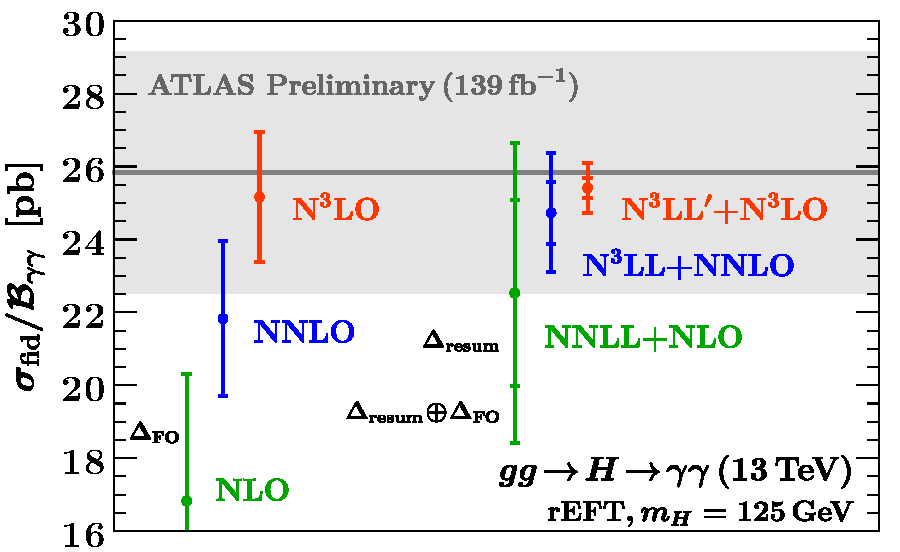
\includegraphics[width=.7\textwidth]{figures/total_xs_fid}
		\caption{ The total fiducial cross-section for the final state  $ gg \to h \to \gamma \gamma$ at both fixed and resumed third order compared to the experimental ATLAS measurement~\cite{ATLAS:2019jst} this figure is taken from~\cite{Billis:2021ecs} \label{fig:ggFxs} }
	\end{center}
\end{figure}
The predictions can be further improved by the computation of mixed QCD-EW effects. Alas, these computations invokes three-loop integrals with both gluons and EW bosons, computed in~\cite{Bonetti:2017ovy} or two-loop ones with two particle final states appearing in the real corrections with the process $ gg \to hg$ computed in~\cite{Bonetti:2020hqh} using differential equations. The computation was completed by inclusion of light quark initial states for the real corrections in~\cite{Becchetti:2020wof} with exact quark mass dependence, reducing the EW uncertainty from $2\%$ to $ \sim 0.6\%$.  \\ The computation of the three-loop form-factors with full top-mass dependence  has been achieved in~\cite{Czakon:2020vql,Czakon:2021yub} correction the cross-section by $-0.26\%$. However, there remains an intricate interplay between the mass effects of $gg$, $qg$ and $qq$ initial states for the real matrix elements that cannot be fully controlled due to the light quark mass effects. \\ NLO corrections to the $h +j$ and $ h+2j$ processes were computed by~\cite{Maltoni:2014eza} in the FT approximation, which used exact born and real correction amplitudes, and approximates the two-loop virtuals by
\begin{equation}
|	\mathcal A^{\mathrm{2-loop}}(m_t,\mu_R^2) |^2 \approx  |	\mathcal A^{\mathrm{1-loop}}(m_t\to \infty,\mu_R^2) |^2\, \frac{|	\mathcal A^{\mathrm{1-loop}}(m_t) |^2}{A^{\mathrm{(0)}}(m_t)\to \infty |^2}. 
\end{equation}
Although this approximation works very well even for $ \pt \gg m_t$, the full top mass effects computations have been carried out in~\cite{Kudashkin:2017skd,Lindert:2018iug,PhysRevLett.120.162001} using the high energy expiation technique. 
\subsection{Vector boson fusion}
The VBF channel has a very distinctive signature, making it very suitable channel for Higgs signal extraction. The suppressed colour exchange between the quarks result in a little jet activity in the central rapidity region, and the quarks will be scattered resulting in two forward jets. The decay products of the Higgs are found in the region between these two forward jets.  These features allows for excellent measurement of Higgs couplings and more difficult decays, and $\mathcal{CP}$ properties determination. Some of these features are also shared with the $Vh$ production channel via Higgs-strahlung. Both of these channels contain the $VVh$ vertex which could be written generally as~\cite{LHCHiggsCrossSectionWorkingGroup:2016ypw}
\begin{equation}
T^{\mu \nu}(p_1,p_2) = a_1 g^{\mu \nu}+ a_2  \left(g^{\mu \nu}- 2\frac{p^\mu_{2} p^\nu }{p_1 \cdot p_2} \right)  + a_3 \frac{p_1^\alpha p_2^ \beta}{p_1 \cdot p_2}\epsilon^{\mu \nu \alpha \beta}. 
\end{equation} 
In the SM only $a_1\neq0$, and the other coefficients represent the anomalous coupling, for example if $a_3 \neq0$ then the Higgs is  $\mathcal{CP}$  odd. The study of the azimuthal angle distribution~$d \sigma_{VBF} / d \Delta \phi_{jj}$ allows for  the determination of these coefficients, with very little dependence on the Higher order corrections on VBF~\cite{hankele2006anomalous}.\\  The NLO QCD inclusive cross-section is known since the 90's~\cite{Han:1992hr}, and later these corrections were made for the differential distributions cf.~\cite{Figy:2003nv,Berger:2004pca}. Unlike the ggF channel, that has an NLO  K-factor of $1.6$ at 13 TeV~\cite{Gomez-Bock:2007azi} , the VBF NLO corrections are small $\sim 10\%$. The two-loop NNLO QCD cross-section has been computed, the most recent is via the structure function approach~\cite{Bolzoni:2010xr} and later in STXS level 1.2 bins with EW corrections~\cite{Denner:2014cla} implemented in an MC generator  \texttt{HAWK}. Despite these corrections being small, they are non-negligible and their inclusion is important for uncertainties reduction.
\subsection{Associated production with EW bosons}
The channels $pp\to Wh/Zh$ are  quark-initiated tree-level processes at LO interpreted as \textbf{Drell-Yan process}~ \cite{Han:1991ia,Brein:2003wg}. These process has been computed up to  NNLO in QCD ($\sim \alpha_s^2$), and  NLO  EW  ($\sim \alpha^2 $)~\cite{Amoroso:2020lgh}.
%%
\par Despite arising for the first time at NNLO in perturbation theory to the partonic cross-section, the gluon fusion channel $g g \rightarrow Zh$ has a non-negligible contribution to the hadronic cross-section~$pp\to Zh$, which could reach $>16\%$ of the total cross-section contribution at $14$ TeV~\cite{Cepeda:2019klc}, see~\autoref{fig:hzratio}. The contribution becomes more significant when looking at large invariant mass bins in the differential cross-section. This is due to the significant abundance of gluons at the LHC for large energy faction~$Q$ as well as the extra enhancement coming from the top quark initiated contribution near the~$t\bar t$ threshold~\cite{Englert:2013vua}.  The gluon fusion channel has a higher scale uncertainties than the quark induced one, as one can see from the uncertainty band of~\autoref{fig:hzratio} predominantly coming from the gluon fusion part~$\sigma_{gg}$.  With that in mind, and the absence of gluon fusion channel for $Wh$ channel, the $Zh$ channel has higher theoretical uncertainties. This further motivates NLO calculation of the  $g g \rightarrow Z h$ channel to higher orders in perturbation theory,  in order to reduce these uncertainties. Facilitating the precision measurement of the $Zh$ channel at the future LHC runs, which in term provides better constraints on several observables, such as sign and magnitude of the top Yukawa coupling,  dipole operators \cite{Englert:2016hvy}.
%%
\begin{figure}
	\begin{center}
		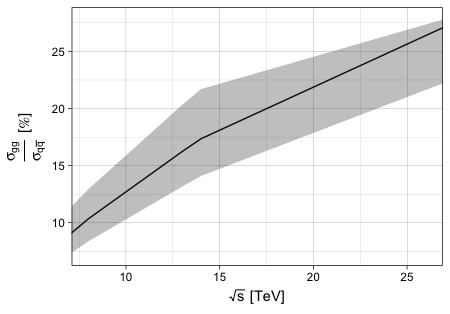
\includegraphics[width=9cm]{./figures/Rplot}
		\caption{The ratio of the $LO$ gluon fusion production cross-section $ gg \to Zh$  ($\sigma_{gg}$) with respect to the $NLO$ Drell-Yan process $ q\bar{q} \to Zh$ cross-section ($\sigma_{q\bar{q}}$) at a $pp$ collider with centre-of-mass energy $\sqrt{s}$. The error band captures the total theoretical uncertainties on both cross-sections dominated by~$\sigma_{gg}$ .}
		\label{fig:hzratio}
	\end{center}
\end{figure}
%%
\par  The leading order (LO) contribution to the $g g \rightarrow Z h$ amplitude, given by one-loop diagrams, was computed exactly in refs.\cite{Kniehl:1990iva, Dicus:1988yh}. However, for the NLO, the virtual corrections contain multi-scale two-loop integrals some of which are still not known analytically ( for the box diagram).  The first computation of the NLO terms has been done by~\cite{Altenkamp:2012sx} using an asymptotic expansion in the limit
$\mt \rightarrow \infty$ and $m_b = 0$, and pointed to a $K$-factor of about $\sim2$.  Later, the computation has been improved via soft gluon resummation, and including NLL terms found in ref.\cite{Harlander:2014wda}, the NLL terms has been matched to the fixed NLO computation of~\cite{Altenkamp:2012sx}.  Top quark mass effects to the  $g g \rightarrow Zh$ process were first implemented using a combination of  large-$\mt$ expansion (LME) and Pad\'e approximants~\cite{Hasselhuhn:2016rqt}. A data-driven approach to extract the gluon fusion dominated non-Drell-Yan part of $Zh$ production using the known relation between  $Wh$
and $ Z h$ associated production when only the Drell-Yan component of the two processes is considered has been investigated in ref.\cite{Harlander:2018yns}. The differential distributions of $g g \rightarrow Zh$  at NLO was studied in ref.\cite{Hespel:2015zea} via LO matrix element matching. 
%%
\par More recent studies of the NLO virtual corrections to this process were based on the high-energy~(HE) expansion improved by Pad\'e approximants with the LME, which extended the validity range of the HE expansion \cite{Davies:2020drs}. However, this expansion is only valid for in the invariant mass region $\sqrt{\hat{s}}  \gtrsim 750\, \si{\GeV} $ and $\sqrt{\hat{s}}  \lesssim 350\,  \si{\GeV}$,  which only covers $\sim 32\%$ of the hadronic cross section. Additionally, numerical computation of the two-loop virtual corrections, though implemented exactly in  \cite{Chen:2020gae}, are rather slow for practical use in MC simulations.  This highlights the importance of an analytical method that can cover the remaining region of the cross-section and can be merged with the HE expansion via Pad\'e approximants. Fortunately, the two-loop corrections to the triangle diagrams can be computed exactly. And the loop integrals appearing in the box correction having no analytic expression can be expanded in small  $Z$ (or Higgs) 
transverse momentum, $\pt$. This method was first used for Higgs pair production in~\cite{Bonciani:2018omm}, to compute the NLO virtual corrections to the box diagrams in the forward kinematics. In~\autoref{chap:hz}, I will discuss the calculation preformed by my collaborators and myself and published in~\cite{Alasfar:2021ppe}, which includes the full top mass dependence of the virtual two-loop correction to~$ gg \to Zh$ in an  analytic form  using the same $\pt$ expansion technique.

\subsection{Associated production with top quarks}
The largest part of the $t\bar t h/th$ uncertainty budget comes from the theoretical modelling of this process's backgrounds, mainly $t \bar t b\bar b,\ t\bar t W$ as backgrounds for $ t\bar t (h \to b\bar b)$ and $ t \bar t ( h \to \mathrm{multileptons})$, respectively. There have been several theoretical developments regarding these backgrounds. Starting with $t\bar t W$, the differential cross-section at NNL+ NLO QCD calculation of this channel has been done in~\cite{Broggio:2019ewu,Kulesza:2020nfh} including EW corrections. The fully decayed final state at NLO QCD~\cite{Bevilacqua:2020pzy,Denner:2020hgg,Bevilacqua:2020srb} and at NLO-EW~\cite{Denner:2021hqi} have been computed. Additionally, these calculations were implemented in~\texttt{POWHEG-BOX}~\cite{Cordero:2021iau}. The comparison between the NLO-QCD with parton showering vs on-shell can be found in~\cite{Bevilacqua:2021tzp}. As for ~$t \bar t b\bar b$, the progress in obtaining higher order corrections is faced with challenges posed by the complexity of this channel. However, progress has been made, for instance the off-shell effects in the fully decayed $ pp \to 2 \ell 2 \nu  4 b$ with NLO corrections was studied in~\cite{Denner:2020orv,Bevilacqua:2021cit}. Further discussion of the theoretical developments of these channels is beyond the scope of this thesis. \\
Regarding the higher order corrections to the $t\bar t h /t h$ channel itself, the NLO QCD+EW effects on the off-shell multileptons final state  were studied in~\cite{Denner:2019zdz},  while the NLO corrections including SMEFT operators were calculated in\cite{Maltoni:2016yxb}. The NLO QCD+EW with parton showering is available in all event generators, and the SMEFT operators at NLO are available in \texttt{MadGraph5\_aMC@NLO} .  As of the time of writing this thesis, there is no NNLO calculation of $t\bar t h /t h$ available. 
%\section{Higgs pseudo-observables \label{sec:higgspos}  }

\section{Concluding remarks \label{sec:singlehiggsconc}  }
The precise determination of the Higgs boson properties is one of the main focus of the Large Hadron Collider (LHC) physics programme. In order to achieve precision-level Higgs measurements both experimental and theoretical uncertainties need to be improved. Though the first can be improved with Higher luminosities and energies, better detectors and improved analysis techniques. Theoretical uncertainties require higher-order calculations, inclusion of mixed EW and QCD terms , inclusion of mass effects and suitable parton distribution functions with Higher order in QCD.  As we have seen, a lot of effort is being put into improving the theoretical predictions of Higgs production channels. Moreover, many computer tools have been made available to compute these cross-sections, for example  \texttt{iHixs2}~\cite{Dulat:2018rbf} or to generate full events, like \texttt{POWHEG}~\cite{Alioli:2008tz,Nason:2009ai,Bagnaschi:2011tu,Campbell:2012am,Luisoni:2013cuh,Jager:2014vna,Hartanto:2015uka} and \texttt{MadGraph5\_aMC@NLO}~\cite{Alwall:2014hca}, and many others can be found with greater detail in the Higgs cross-sections working group~\cite{HXSWG}.  \\ Sometimes, to improve the measurement of the process, it is not sufficient to only improve the theoretical prediction of the channel itself, but also its backgrounds, which is particularly important for $t\bar th $. Hence, higher order calculations of processes like $t\bar t W$ with parton-shower effects as well as improved analysis to distinguish $t\bar t(h \to b \bar b) $ have a significant impact on  $t\bar th $ measurements.
Event generator tools with SMEFT implementation in Higgs processes with patron showing interface capabilities  have been implemented in a \texttt{MadGraph5\_aMC@NLO} model~\texttt{SMEFTatNLO}~\cite{Degrande:2020evl} which enabled loop computations with SMEFT operators and consequently fits of the SMEFT Wilson coefficients with Higgs data at NLO as we have seen in~\autoref{chap:HiggsEFT}.\\
There is plenty of room for future improvements in the reduction of theory uncertainty budget, and providing better theoretical prediction of the Higgs processes in the SM and beyond. From inclusion of patron shower matching , merging and validation to  inclusion of two-loop calculations of gluon fusion $Zh$  and EW NLO effects of  $t\bar th $, all in preparation to the HL-LHC Higgs precision era ! 

%%%
%\begin{figure}
%	\begin{center}
%		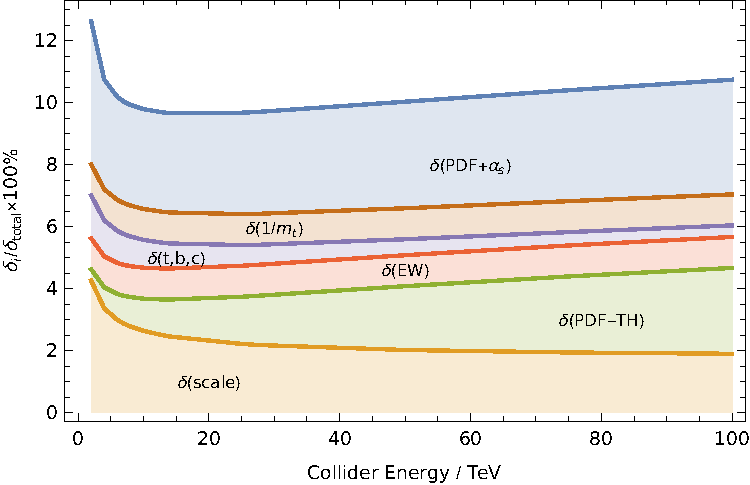
\includegraphics[width=9cm]{./figures/error_plot}
%		\caption{The error budget plot showing the cumulative uncertainty of the total Higgs cross-section via gluon fusion at ~N$\,^3$LO as a function of energy. This plot is taken from~\cite{Dulat:2018rbf}}
%		\label{fig:error-budget}
%	\end{center}
%\end{figure}
%%%


%
%\subsubsection{The LO amplitude}
%We recall the projected LO on shell amplitude~\cite{Gunion:1989we}
%\begin{equation}
%	\mathcal{M}_{LO} = \frac{ T_f \alpha_s \ght }{2 \sqrt{2} \pi } \mathcal F^{(1 \ell)}  S_\epsilon ,
%\end{equation}
%with the projector
%\begin{equation}
%	\mathbb{P}^{\mu \nu} = g^{\mu \nu}- 2\frac{p^\mu_{2} p^\nu }{m_h^2},
%\end{equation}
%and the 1 loop form factor
%\begin{align}
%	\mathcal F^{(1 \ell)} &= m_h\,\sqrt{\tau} \left( (1-\tau) H(0,0,x)+2\right) ,\nonumber  \\
%	x &= \frac{\tau+2 \sqrt{1-\tau}-2}{\tau},
%	\label{f1l}
%\end{align}
%where $ \tau = 4 m_t^2/m_h^2$,  $H(m,n,x)$ is the harmonic ploylogarithm function~(HPL), and
%\begin{equation}
%	S_\epsilon = \Gamma(1+\epsilon) (\mu/m_t)^{2\epsilon}.
%\end{equation}
%\\
%The decay width is therefore given by
%\begin{equation}
%	\Gamma_{LO}(h\to gg) = \frac{\alpha_s^2\, G_F\,m_h^3 \,m_t^2\,\tau }{8 \pi^3 \sqrt{2}}  \, \left( 3(\tau-1)^2 H(0,0,0,0,x)+2(\tau-1)H(0,0,x)+2\right)
%\end{equation}
%With the following definitions
%\begin{align}
%	\ght &=\ght^{SM} = {\sqrt{2} m_t \over v}, \nonumber \\
%	v &= \left( G_F \sqrt{2}\right) ^{-1/2}, \nonumber \\
%	T_f &= \frac{1}{2} .
%\end{align}